% TEMPLATE INSTRUCTIONS
% Fill in the information in template/information.tex
% The front matter (abstract and acknowledgements) needs slight modification for Bachelor theses.

% IMPORT SETTINGS
\documentclass[12pt, a4paper, twoside, openright]{report}
% GENERAL
\newcommand{\thesisType}{M} % M - master, B - bachelor
\newcommand{\thesisAuthor}{Name Familyname}
\newcommand{\thesisMonth}{\monthname}
\newcommand{\thesisYear}{\the\year}

% LAYOUT
\newcommand{\thesisLayout}{2} % One-sided (1) or two-sided (2) layout
% Note: \cleardoublepage is redefed to \clearpage for one-sided layout

% Controls e.g. todonotes
\newcommand{\thesisStatus}{d} % d for draft, f for final

% TITLE (cover page & title page, imprint page; possibly different line breaks)
\newcommand{\thesisTitle}{An Informative Headline describing \\[0.2cm] the Content of the Report}
\newcommand{\thesisImprintTitle}{An Informative Headline describing the Content of the Report}


% SUBTITLE (cover page & title page, imprint page; possibly different line breaks)
\newcommand{\thesisSubtitle}{A Subtitle that can be Very Much Longer if Necessary}
\newcommand{\thesisImprintSubtitle}{A Subtitle that can be Very Much Longer if Necessary}


% PROGRAMME, DEPARTMENT, DIVISION, RESEARCH GROUP AND UNIVERSITY INFO
\newcommand{\thesisMasterProgramme}{Master Programme Name}  % "Master's thesis in \thesisMasterProgramme"

\newcommand{\thesisDepartment}{Department of Some Subject or Technology}
\newcommand{\thesisDivision}{Division of Division name}
\newcommand{\thesisGroup}{Name of research group (if applicable)}

\newcommand{\thesisUniversity}{Chalmers University of Technology}
\newcommand{\thesisUniversityURL}{www.chalmers.se}
\newcommand{\thesisCity}{Gothenburg}
\newcommand{\thesisCountry}{Sweden}
\newcommand{\thesisLocation}{\thesisCity, \thesisCountry}


% MORE IMPRINT PAGE INFO
\newcommand{\thesisSupervisor}{Name, Company or Department}
\newcommand{\thesisExaminer}{Name, Department}
\newcommand{\thesisPrintedBy}{Chalmers Reproservice} % remove this line to remove it on the imprint page

\newcommand{\thesisImprintLocation}{SE-412 96 Gothenburg}
\newcommand{\thesisUniversityTel}{+46 31 772 1000}


% COVER FIGURE
% Remove the following line to remove the figure
\newcommand{\thesisCoverFigure}{frontmatter/Wind.png}
% Caption for cover page figure if used, possibly with reference to further information in the report:
\newcommand{\thesisCoverFigureCaption}{Wind visualization constructed in Matlab showing a surface of constant wind speed along with streamlines of the flow.}

% BASIC SETTINGS
%%%%%%%%%%%%%%%%%%%%%%%%%%%%%%%%%%%%%%%%%%%%%%%%%%%%%%%%%%%%%%%%%%%%%
\usepackage[UKenglish]{babel}		% Language settings
\usepackage[utf8]{inputenc}			% Input settings
\usepackage[T1]{fontenc}			% Output settings
\usepackage{lmodern}				% Latin modern font
\usepackage{textcomp}				% Fonts, symbols etc.
\usepackage[top=3cm, bottom=3cm, inner=3cm, outer=3cm]{geometry}

%%%%%%%%%%%%%%%%%%%%%%%%%%%%%%%%%%%%%%%%%%%%%%%%%%%%%%%%%%%%%%%%%%%%%
% MATHS
\usepackage{amsmath}				% Mathematical expressions
\usepackage{amssymb}				% Mathematical symbols
\usepackage{mathtools}              % (TODO)
\usepackage{commath}                % E.g. \abs{} och \norm{}
\usepackage{dsfont}                 % (TODO)
\usepackage{bm}                     % Bold math symbols
\usepackage{gensymb}                % (TODO)
\usepackage{mathrsfs}               % (TODO)

%%%%%%%%%%%%%%%%%%%%%%%%%%%%%%%%%%%%%%%%%%%%%%%%%%%%%%%%%%%%%%%%%%%%%
% FIGURES
\usepackage{graphicx}				% Figures
\usepackage{float} 					% Position enforcement using [H]
\usepackage{pdfpages}               % Include PDF-pages

%%%%%%%%%%%%%%%%%%%%%%%%%%%%%%%%%%%%%%%%%%%%%%%%%%%%%%%%%%%%%%%%%%%%%
% TABLES
\usepackage{array}                  % (TODO)
\usepackage{tabularx}               % (TODO)
\usepackage{diagbox}                % Slash in tables
\usepackage{booktabs}               % Improved rules in tables

% Reduce weight of top and bottom rules
\setlength{\heavyrulewidth}{0.075em}

% TABLE LAYOUT (optional)
%\newcommand{\PreserveBackslash}[1]{\let\temp=\\#1\let\\=\temp}
%\newcolumntype{C}[1]{>{\PreserveBackslash\centering}p{#1}}
%\newcolumntype{R}[1]{>{\PreserveBackslash\raggedleft}p{#1}}
%\newcolumntype{L}[1]{>{\PreserveBackslash\raggedright}p{#1}}

%%%%%%%%%%%%%%%%%%%%%%%%%%%%%%%%%%%%%%%%%%%%%%%%%%%%%%%%%%%%%%%%%%%%%
% CAPTION LAYOUT
\usepackage[
    labelfont       = bf,
    font            = normalsize,
    width           = 0.92\textwidth,
    justification   = justified,
    singlelinecheck = true
]{caption}
% NOTE: Consider matching the caption font size (normalsize above)
% to the font size in the figure/table. \captionsetup can be used
% to change settings locally.

% Caption for subfigures (optional)
% \usepackage{subcaption}

% \DeclareCaptionLabelFormat{r-parens}{#2)} %Define our custom label
% \captionsetup[subfigure]{font=scriptsize, textfont=sl,%
% labelformat=r-parens, width=0.8\textwidth, position=b}

%%%%%%%%%%%%%%%%%%%%%%%%%%%%%%%%%%%%%%%%%%%%%%%%%%%%%%%%%%%%%%%%%%%%%
% CITATIONS/BIBLIOGRAPHY
\usepackage{silence}  % Suppress warnings (manually)
\WarningFilter{biblatex}{File 'english-ieee.lbx'}

\usepackage[
    backend     = biber,
    style       = ieee,
    dashed      = false,
    maxnames    = 6,
    natbib      = true,
    date        = iso,
    urldate     = iso,
    seconds     = true
]{biblatex}

\DefineBibliographyStrings{english}{%
  mathesis = {MSc thesis},
}
\renewcommand{\subtitlepunct}{\addcolon\addspace}

\addbibresource{references.bib}

%%%%%%%%%%%%%%%%%%%%%%%%%%%%%%%%%%%%%%%%%%%%%%%%%%%%%%%%%%%%%%%%%%%%%
% SI UNITS
\usepackage{siunitx}

\sisetup{output-decimal-marker={.}}
\sisetup{exponent-product={\cdot}}
\sisetup{range-phrase=--}
\sisetup{per-mode=symbol}
\sisetup{separate-uncertainty=true}
%\sisetup{round-mode=places,round-precision=3}
%\sisetup{parse-numbers = false}

%Speed of light and eV per speed of light
\DeclareSIUnit\clight{\text{\ensuremath{c}}}
\DeclareSIUnit\eVperc{\eV\per\clight}
\DeclareSIUnit\au{\text{a.u.}}

%%%%%%%%%%%%%%%%%%%%%%%%%%%%%%%%%%%%%%%%%%%%%%%%%%%%%%%%%%%%%%%%%%%%%
% HEADER & FOOTER LAYOUT
\usepackage{fancyhdr}
\usepackage{chappg}

\pagestyle{fancy}
\setlength{\headheight}{15pt}  % Suppress warning
\renewcommand{\chaptermark}[1]{\markboth{\thechapter.\space#1}{}}

\if\thesisLayout 1 % One-sided
    \fancyhf{}
	\fancyhead[L]{\nouppercase{ \leftmark}}
	\fancyhead[R]{\nouppercase{ \rightmark}}
	\fancyfoot[C]{\thepage}
\fi

\if\thesisLayout 2 % Two-sided
  	\fancyhf{}
	\fancyhead[LE]{\nouppercase{ \leftmark}}
	\fancyhead[RO]{\nouppercase{ \rightmark}}
	\fancyfoot[LE,RO]{\thepage}
	\fancypagestyle{plain}{% Redefine the plain page style
	\fancyhf{}
	\renewcommand{\headrulewidth}{0pt}
	\fancyfoot[LE,RO]{\thepage}}
\fi

%%%%%%%%%%%%%%%%%%%%%%%%%%%%%%%%%%%%%%%%%%%%%%%%%%%%%%%%%%%%%%%%%%%%%
% FOOTNOTE LAYOUT
\usepackage[bottom, hang]{footmisc}
% The multiple option does not seem to work. It should produce commas
% between markers in cases like "Lipsum\footnote{Foo}\footnote{Bar}".
% For now, use the following:
\newcommand{\footnotemarksep}{\textsuperscript{,}}
% A better approach might be: https://tex.stackexchange.com/a/62091

% Change the width of the ruler above footnotes:
\renewcommand*\footnoterule{\rule[2pt]{\textwidth}{0.5pt}}

% Space before footnote text (0pt for marker width):
\setlength{\footnotemargin}{0pt}

% Might be preferable for multi-paragraph footnotes:
%\setlength{\footnotesep}{\baselineskip}

% For footnote symbols instead of numbers, use options symbol*
% and perpage with footmisc.
% To change symbol set, use e.g.: \setfnsymbol{wiley}

%%%%%%%%%%%%%%%%%%%%%%%%%%%%%%%%%%%%%%%%%%%%%%%%%%%%%%%%%%%%%%%%%%%%%
% BLANK LINE AND SPACING
\usepackage[raggedright]{titlesec}
\usepackage{parskip}				% Enables vertical spaces correctly

\setlength{\parindent}{0pt}
\setlength{\parskip}{\baselineskip}

% Title spacing

% Defaults:
%\titlespacing*{\chapter} {0pt}{50pt}{40pt}
%\titlespacing*{\section} {0pt}{3.5ex plus 1ex minus .2ex}{2.3ex plus .2ex}
%\titlespacing*{\subsection} {0pt}{3.25ex plus 1ex minus .2ex}{1.5ex plus .2ex}
%\titlespacing*{\subsubsection}{0pt}{3.25ex plus 1ex minus .2ex}{1.5ex plus .2ex}
%\titlespacing*{\paragraph} {0pt}{3.25ex plus 1ex minus .2ex}{1em}
%\titlespacing*{\subparagraph} {\parindent}{3.25ex plus 1ex minus .2ex}{1em}

\setlength{\belowdisplayskip}{0pt}
\setlength{\belowdisplayshortskip}{0pt}
\setlength{\abovedisplayskip}{0pt}
\setlength{\abovedisplayshortskip}{0pt}

\raggedbottom % does not fill the entire page if not necessary

%%%%%%%%%%%%%%%%%%%%%%%%%%%%%%%%%%%%%%%%%%%%%%%%%%%%%%%%%%%%%%%%%%%%%
% TITLE AND TOC LAYOUT
\usepackage{titletoc}
\usepackage[title]{appendix}

% Define the number of section levels to be included in toc and numbered
\setcounter{tocdepth}{3}
\setcounter{secnumdepth}{3}

% Chapter styles (NOTE: only the last one is used)
\newcommand*{\thesisChapterStyle}{1} % 0 for default

\ifnum\thesisChapterStyle=1
    \titleformat{\chapter}[hang]{\fontsize{30}{10}\selectfont}
    {{\fontsize{30pt}{1em}\vspace{-5.2ex}\selectfont \textnormal{\thechapter. \hspace{1pt}}}}
    {.5ex}{\raggedright}[\rule{\textwidth}{0.3pt}]
    \titlespacing{\chapter}{0pt}{0pt}{\parskip}
\fi

\ifnum\thesisChapterStyle=2
    \titleformat{\chapter}[display]
    {\Huge\bfseries\filcenter}
    {{\fontsize{50pt}{1em}\vspace{-4.2ex}\selectfont \textnormal{\thechapter}}}{1ex}{}[]
\fi

% Handle number of blank pages at chapter break
\if\thesisLayout 1
    \renewcommand{\cleardoublepage}{\clearpage}
\fi

% Name of chapters
% \addto\captionsenglish{\renewcommand{\abstractname}{}}
\addto{\captionsenglish}{\renewcommand{\contentsname}{Table of Contents}}
% \addto\captionsenglish{\renewcommand{\appendixname}{}}

% \bibname seems to be reset at \begin{document} (workaround in main)
\newcommand{\thesisBibName}{References}
\addto{\captionsenglish}{\renewcommand{\bibname}{\thesisBibName}}

%%%%%%%%%%%%%%%%%%%%%%%%%%%%%%%%%%%%%%%%%%%%%%%%%%%%%%%%%%%%%%%%%%%%%
% COVER PAGE BACKGROUND
\usepackage{eso-pic}

\newcommand{\backgroundpic}[3]{
	\put(#1,#2){
	\parbox[b][\paperheight]{\paperwidth}{
	\centering
	\includegraphics[width=\paperwidth,height=\paperheight,keepaspectratio]{#3}}}}

% COLOUR FOR HEADERS
\definecolor{headerBrown}{RGB}{144,102,78}

\if\thesisType B
    \definecolor{thesisHeaderColor}{RGB}{126,180,56} % Green
\fi

\if\thesisType M
    \definecolor{thesisHeaderColor}{cmyk}{0.14,0,0,0.65} % Gray
\fi

%%%%%%%%%%%%%%%%%%%%%%%%%%%%%%%%%%%%%%%%%%%%%%%%%%%%%%%%%%%%%%%%%%%%%
% PATCHES AND FIXES

% Give error on include with missing file
\makeatletter
\patchcmd\@include\@input@\input{}{}
\makeatother

%%%%%%%%%%%%%%%%%%%%%%%%%%%%%%%%%%%%%%%%%%%%%%%%%%%%%%%%%%%%%%%%%%%%%
% OTHER
\usepackage{csquotes}               % Quotations, using the command
\usepackage{lipsum}                 % Generating Lorem Ipsum
\usepackage{enumitem}               % Provides control over lists
\usepackage{xcolor}                 % Coloured text

\usepackage[yyyymmdd]{datetime}     % Dates
\renewcommand{\dateseparator}{-}    % Modify date separator

% To-do notes
\if\thesisStatus f
    \usepackage[textsize=tiny,disable]{todonotes}
\else
    \if\thesisStatus d
        \usepackage[textsize=tiny]{todonotes}
    \fi
\fi
\setlength{\marginparwidth}{2.5cm}

%%%%%%%%%%%%%%%%%%%%%%%%%%%%%%%%%%%%%%%%%%%%%%%%%%%%%%%%%%%%%%%%%%%%%
% REFERENCES
% hyperref should, in general, be loaded last to avoid problems.
% Hence, other packages should, most likely, be placed above this.

\if\thesisStatus f
    \newcommand{\thesisColorlinks}{false}
\else
    % change to false for black links in draft
    \newcommand{\thesisColorlinks}{true}
\fi

% Clickable links in final pdf
\usepackage[
    hidelinks,
    linktoc     = all,
    colorlinks  = \thesisColorlinks,
    filecolor   = blue,
    linkcolor   = blue,
    urlcolor    = blue,
    citecolor   = blue,
    anchorcolor = blue,
]{hyperref}
\usepackage{url}                                        % Clickable url links
\usepackage[capitalise,noabbrev,nameinlink]{cleveref}   % Clever references
% optional: [nameinlink], makes e.g. "Table" part of the link
% Note: use \cpageref to reference pages with correct hyperlinks

% CREF
\crefname{equation}{}{}  % "(1.1)" instead of "Equation (1.1)"

% NUMBERING:
\numberwithin{equation}{chapter}    % Numbering order for equations
\numberwithin{figure}{chapter}	    % Numbering order for figures
\numberwithin{table}{chapter}		% Numbering order for tables

% OPTIONAL PACKAGES AND SETTINGS
%%%%%%%%%%%%%%%%%%%%%%%%%%%%%%%%%%%%%%%%%%%%%%%%%%%%%%%%%%%%%%%%%%%%%
% NOTE: as hyperref should, in general, be loaded last, it is
%   recommended that used packages are moved from here to basic.tex

%%%%%%%%%%%%%%%%%%%%%%%%%%%%%%%%%%%%%%%%%%%%%%%%%%%%%%%%%%%%%%%%%%%%%
% \usepackage[export]{adjustbox}    % Alt. way of inserting subfigs
% \usepackage{multicol}             % Multiple columns

% \usepackage{marvosym}             % Symbols, e.g. euro, zodiac etc.
% \usepackage{helvet}				% Enables different fonts
% \usepackage{wrapfig}              % Wrap figures
% \usepackage{arydshln}             % Dashed \hline and other

% \usepackage{mhchem}               % Isotopes
% \usepackage{chemfig}				% Chemical structures

% \usepackage{pdflscape}            % Landscape-mode
% \usepackage{verbatim}             % e.q. comment environment
% \usepackage{moreverb}				% List settings
% \usepackage{comment}              % comment environment


%%%%%%%%%%%%%%%%%%%%%%%%%%%%%%%%%%%%%%%%%%%%%%%%%%%%%%%%%%%%%%%%%%%%%
% Only show equations if referred :
% \mathtoolsset{showonlyrefs}    % Don't work with cref
% \usepackage{autonum}           % Don't work with biblatex

%%%%%%%%%%%%%%%%%%%%%%%%%%%%%%%%%%%%%%%%%%%%%%%%%%%%%%%%%%%%%%%%%%%%%
% LINE SPACING
%\usepackage{setspace}              % (TODO)
%\setstretch{1.2}
%\linespread{1.2}

%\usepackage{color, colortbl}       % Colors in tables etc.


%%%%%%%%%%%%%%%%%%%%%%%%%%%%%%%%%%%%%%%%%%%%%%%%%%%%%%%%%%%%%%%%%%%%%
% TIKZ
% \usepackage{tikz}                   % Tikz figures
% \usepackage[RPvoltages]{circuitikz} % CircuiTikz
% \usepackage{pgf,pgfplots}           % Pgfplots
%%%%%%%%%%%%%%%%%%%%%%%%%%%%%%%%%%%%%%%%%%%%%%%%%%%%%%%%%%%%%%%%%%%%%
% PGFPLOT
% \usetikzlibrary{patterns, arrows.meta ,fit, positioning, shapes}

% \pgfplotsset{compat=1.14}

% \pgfplotsset{every axis/.append style={
%     scaled y ticks = false,
%     scaled x ticks = false,
%     y tick label style={/pgf/number format/.cd, fixed, fixed zerofill,
%                         int detect,1000 sep={\;},precision=3},
%     x tick label style={/pgf/number format/.cd, fixed, fixed zerofill,
%                         int detect, 1000 sep={},precision=3}
% }
% }

%%%%%%%%%%%%%%%%%%%%%%%%%%%%%%%%%%%%%%%%%%%%%%%%%%%%%%%%%%%%%%%%%%%%%
% CODE
\usepackage{listings}  % Enables source code listings

% \definecolor{listinggray}{gray}{0.98}
% \definecolor{lbcolor}{rgb}{0.98,0.98,0.98}
% \lstset{
% 	backgroundcolor=\color{lbcolor},
% 	tabsize=4,
% 	rulecolor=,
% 	language=matlab,
%     basicstyle=\scriptsize\ttfamily,
%     upquote=true,
%     aboveskip={1.5\baselineskip},
%     columns=fixed,
%     showstringspaces=false,
%     extendedchars=true,
%     breaklines=true,
%     prebreak = \raisebox{0ex}[0ex][0ex]{\ensuremath{\hookleftarrow}},
%     frame=single,
%     showtabs=false,
%     showspaces=false,
%     showstringspaces=false,
%     identifierstyle=\ttfamily,
%     keywordstyle=\color[rgb]{0,0,1},
%     commentstyle=\color[rgb]{0.133,0.545,0.133},
%     stringstyle=\color[rgb]{0.627,0.126,0.941},
% }

%%%%%%%%%%%%%%%%%%%%%%%%%%%%%%%%%%%%%%%%%%%%%%%%%%%%%%%%%%%%%%%%%%%%%
% MODIFY TOLERANCES
%\pretolerance=1100
%\tolerance=8000
%\emergencystretch=0pt

%\righthyphenmin=4
%\lefthyphenmin=4
\setcounter{biburlnumpenalty}{100}
\setcounter{biburlucpenalty}{100}
\setcounter{biburllcpenalty}{100}

% USER DEFINED COMMANDS:
%%%%%%%%%%%%%%%%%%%%%%%%%%%%%%%%%%%%%%%%%%%%%%%%%%%%%%%%%%%%%%%%%%%%%

% Really wide (adpative) hat
%\usepackage{scalerel,stackengine}
%\stackMath
%\newcommand*\reallywidehat[1]{\savestack{\tmpbox}{\stretchto{%
%\scaleto{\scalerel*[\widthof{\ensuremath{#1}}]{\kern.1pt\mathchar"0362\kern.1pt}%
%{\rule{0ex}{\textheight}}}{\textheight}}{2.4ex}}\stackon[-6.9pt]{#1}{\tmpbox}}

% Scientific notation with round-precision
%\newcommand*{\numsc}[2]{\num[scientific-notation=true, round-mode=places, round-precision=#2]{#1}}

\renewcommand*{\i}{\mathrm{i}}      % Imaginary unit
\newcommand*{\e}{\mathrm{e}}        % Euler's number
\renewcommand*{\d}{\mathrm{d}}      % Differential d

% Do not adjust parenthesis size automatically in the following
\renewcommand{\exp}{\operatorname{exp}}


% CHOOSE SUBSET OF FILES TO COMPILE (USES OLD .aux FILES)
% Sometimes, this will cause a blank page at the beginning.
% One way to fix this is to add \cleardoublepage at the end of every
% included file.
\if\thesisStatus d % only effective in draft mode
    % \includeonly{chapters/methods}
\fi

\begin{document}

% COVER PAGE, TITLE PAGE AND IMPRINT PAGE
\if\thesisStatus f
    \pagenumbering{alph}
    % COVER PAGE
{ % make parskip changes local
\ifx\thesisType\undefined
Undefined Thesis type in settings.tex
\else
  \if\thesisType M
    \else
    \if\thesisType B
    \else
    Define \textbackslash ThesisType as M for master's thesis or B for bachelor thesis in project\_information.tex
    \fi
  \fi
\fi

% COVER PAGE
\begin{titlepage}
\newgeometry{top=3cm, bottom=1cm,
			left=2.25 cm, right=2.25cm}	% Temporarily change margins

%Header Front Page
\ifx\thesisType\undefined
\else
    \if\thesisType M
    \vtop{
        \null\vspace{-25mm}
        \centerline{
\includegraphics[width=1.18\textwidth]{template/figures/GrayHeaderPattern.jpg}}
        \vspace{-2.3cm}
        \hbox{\hspace{0mm}
\includegraphics[height=18mm]{template/figures/AvancezChalmersU_white_right.eps}}
        \centerline{\textcolor{headerBrown}{\rule{1.18\textwidth}{4pt}}}
        \vspace{\paperheight}\vspace{-85mm}
        \centerline{\textcolor{thesisHeaderColor}{\rule{1.1\textwidth}{0.8pt}}} % Rule after Department
        \vspace{-\paperheight}\vspace{85mm}
    }
    \fi
    \if\thesisType B
    \vtop{
        \null\vspace{-25mm}
        \centerline{
\includegraphics[width=1.18\textwidth,height=80pt]{template/figures/GreenHeaderPattern.jpg}}
        \vspace{-2.3cm}
        \hbox{\hspace{0mm}
\includegraphics[height=18mm]{template/figures/AvancezChalmers_white_right.eps}}
        \centerline{\textcolor{headerBrown}{\rule{1.18\textwidth}{4pt}}}
        \vspace{\paperheight}\vspace{-85mm}
        \centerline{\textcolor{thesisHeaderColor}{\rule{1.1\textwidth}{0.8pt}}} % Rule after Department
        \vspace{-\paperheight}\vspace{85mm}
    }
    \fi
\fi

% Cover picture
\ifx\thesisCoverFigure\undefined
\else
    \begin{figure}[H]
    \centering
    \vspace{1cm}	% Adjust vertical spacing here
    \includegraphics[width=0.9\linewidth]{\thesisCoverFigure}
    \end{figure}
\fi

% Cover text
\mbox{}
\vfill
\renewcommand{\familydefault}{\sfdefault} \normalfont % Set cover page font
\textbf{{\Huge 	\thesisTitle}} 	\\[0.5cm]
{\Large \thesisSubtitle}\\[0.4cm]
\if\thesisType M
    Master's thesis in
\else
    Kandidatarbete i
\fi
\thesisMasterProgramme \setlength{\parskip}{1cm}


\noindent
{\Large \MakeUppercase{\thesisAuthor}}
\setlength{\parskip}{1.5cm} % NOTE: 1cm (1.5cm) with (without) division (below department)
\ifx\thesisCoverFigure\undefined
    \vspace{6cm}  % increase space if there is no figure
\fi

\noindent
\textcolor{thesisHeaderColor}{\small\textbf{\MakeUppercase{\thesisDepartment}}}
\setlength{\parskip}{1mm}

{\small \MakeUppercase{\thesisUniversity}} \\
{\small \thesisLocation\ \thesisYear \\
\href{\thesisUniversityURL}{\textcolor{black}{\thesisUniversityURL}}}\vspace{1.7cm}

\renewcommand{\familydefault}{\rmdefault} \normalfont % Reset standard font
\end{titlepage}
\restoregeometry

% BACK OF COVER PAGE (BLANK PAGE)
\if\thesisLayout 2
\newpage
\thispagestyle{empty}
\mbox{}
\fi
}

\fi
\pagenumbering{roman}
% TITLE PAGE
{ % make parskip changes local
\newpage
\thispagestyle{empty}
\begin{center}
	\textsc{\large
	\if\thesisType M
	    Master's thesis
	\else
	    Kandidatarbete
	\fi
	\thesisYear
	}\\[4cm]
	\textbf{\Large \thesisTitle} \\[1cm]
	{\large \thesisSubtitle}\\[1cm]
	{\large \thesisAuthor}

	\vfill
	% Logotype on titlepage
	\begin{figure}[H]
	\centering
	% Remove this figure to remove the titlepage logotype
	\if\thesisType M
    
\includegraphics[width=0.2\pdfpagewidth]{template/figures/AvancezChalmersU_black_centered.eps} \\
    \fi
    \if\thesisType B
    
\includegraphics[width=0.2\pdfpagewidth]{template/figures/AvancezChalmers_black_centered.eps} \\
    \fi
	\end{figure}	\vspace{5mm}

	\thesisDepartment\\
	\emph{\thesisDivision}\\
	\ifx\thesisGroup\undefined
    \else
    \thesisGroup\\
    \fi
	\textsc{\thesisUniversity}\\
	\thesisLocation\ \thesisYear\\
\end{center}
}

\if\thesisStatus f
    % IMPRINT PAGE (BACK OF TITLE PAGE)
{ % make parskip changes local
\newpage
\thispagestyle{empty}
\vspace*{4.5cm}
\thesisImprintTitle\\
\thesisImprintSubtitle\\
\thesisAuthor \setlength{\parskip}{1cm}

\copyright~\thesisAuthor, \thesisYear. \setlength{\parskip}{1cm}

\if\thesisType M
    Advisor:
\fi
\thesisAdvisor\\
\if\thesisType M
    Supervisor:
\else
    Handledare:
\fi
\thesisSupervisor\\
\if\thesisType M
    Examiner:
\else
    Examinator:
\fi
\thesisExaminer \setlength{\parskip}{1cm}

\if\thesisType M
    Master's Thesis
\else
    Kandidatarbete
\fi
\thesisYear\\
\thesisDepartment\\
%\thesisDivision\\
\ifx\thesisGroup\undefined
\else
\thesisGroup\\
\fi
Chalmers University of Technology and University of Gothenburg\\
\thesisImprintLocation\\
\if\thesisType M
    Telephone:
\else
    Telefon:
\fi
\thesisUniversityTel \setlength{\parskip}{0.5cm}

\vfill
\ifx\thesisCoverFigure\undefined
\else
    \if\thesisType M
        Cover:
    \else
        Omslag:
    \fi
    \thesisCoverFigureCaption
    \setlength{\parskip}{0.5cm}
\fi

\if\thesisType M
    Typeset in
\else
    Typsatt i
\fi
\LaTeX\\
\ifx\thesisPrintedBy\undefined
\else
    \if\thesisType M
        Printed by
    \else
        Tryckt av
    \fi
    \thesisPrintedBy\\
\fi
\thesisLocation\ \thesisYear
}

\fi

% ABSTRACT & ACKNOWLEDGEMENTS
\thesisImprintTitle\\
\thesisImprintSubtitle\\
\thesisAuthor\\
\thesisDepartment\\
\thesisUniversity\setlength{\parskip}{0.5cm}

\thispagestyle{plain}			% Suppress header
\section*{\abstractname}
Lorem ipsum dolor sit amet, consectetur adipisicing elit, sed do eiusmod tempor incididunt ut labore et dolore magna aliqua. Ut enim ad minim veniam, quis nostrud exercitation ullamco laboris nisi ut aliquip ex ea commodo consequat. Duis aute irure dolor in reprehenderit in voluptate velit esse cillum dolore eu fugiat nulla pariatur. Excepteur sint occaecat cupidatat non proident, sunt in culpa qui officia deserunt mollit anim id est laborum.

\vfill
\if\thesisType M
    \textbf{Keywords:}
\else
    \textbf{Nyckelord:}
\fi
lorem, ipsum, dolor, sit, amet, consectetur, adipisicing, elit, sed, do.

\if\thesisLayout 2
\newpage				% Create blank page
\thispagestyle{empty}
\mbox{}
\fi

\thispagestyle{plain}			% Suppress header
\section*{Acknowledgements}
We would first and foremost like to thank our academic supervisor Moa Johansson, who have supported us throughout this work. Giving us excellent advise on everything from structuring the work to writing.

Secondly, we would like to thank all the people at SVEXA for their help and cooperation.
A special thanks to Rickard Nilsson for helping us access the data needed for the project and Mikael Mattsson, Filip Larsen, and Johan Rogestedt for sharing their knowledge of training planning and exercise science.

We would also like to thank Carl-Johan Seger for taking on the role of examiner and for his thoughtful feedback.

A big thanks also to Tobias Karlsson for his feedback, Oskar Eriksson for the early discussions of scheduling problems, and Joel Karlsson for the discussions of sorting and errors.

Last but not least we would like to thank our friends and family for the emotional support during the work of this thesis.

% Johan would also like to thank Rikard for a greater partnership!

\vspace{0.25cm}
\hfill
\thesisAuthor, \thesisCity, \thesisMonth\ \thesisYear

\if\thesisLayout 2
\newpage				% Create blank page
\thispagestyle{empty}
\mbox{}
\fi


% TABLE OF CONTENTS
% Use a separate file to be able to exclude with \includeonly.
\tableofcontents
% The page numbering is changed after this, whence we need a \cleardoublepage.
% We put it here to be able to exclude it with \includeonly.
\cleardoublepage


% BEGINNING OF MAIN DOCUMENT
\pagenumbering{arabic}	% Arabic numbering starting from 1 (one)

% CHAPTERS
\chapter{Introduction}
This chapter presents the section levels that can be used in the template.

\section{Section levels}
The following table presents an overview of the section levels that are used in this document. The number of levels that are numbered and included in the table of contents is set in the settings file \texttt{Settings.tex}. The levels are shown in \cref{sec:introduction_section}\footnote{
Lorem ipsum dolor sit amet, consectetuer adipiscing elit. Ut purus elit, vestibulum ut, placeratac, adipiscing vitae, felis. Curabitur dictum gravida mauris.}%
\footnotemarksep%
\footnote{Lorem ipsum dolor sit amet, consectetuer adipiscing elit. Ut purus elit, vestibulum ut, placeratac, adipiscing vitae, felis. Curabitur dictum gravida mauris.}%
.

\begin{table}[H]
\centering
\begin{tabular}{ll} \hline\hline
Name & Command\\ \hline
Chapter & \textbackslash\texttt{chapter\{\emph{Chapter name}\}}\\
Section & \textbackslash\texttt{section\{\emph{Section name}\}}\\
Subsection & \textbackslash\texttt{subsection\{\emph{Subsection name}\}}\\
Subsubsection & \textbackslash\texttt{subsubsection\{\emph{Subsubsection name}\}}\\
Paragraph & \textbackslash\texttt{paragraph\{\emph{Paragraph name}\}}\\
Subparagraph & \textbackslash\texttt{paragraph\{\emph{Subparagraph name}\}}\\ \hline\hline
\end{tabular}
\end{table}

%\footnote{\lipsum[2]}.

\section{Section} \label{sec:introduction_section}
\subsection{Subsection}
\subsubsection{Subsubsection}
\paragraph{Paragraph}
\subparagraph{Subparagraph}
\subparagraph{Subparagraph 2}
\newpage

\section{Section}
\lipsum[1]
\subsection{Subsection}
\lipsum[2]
\subsubsection{Subsubsection}
\lipsum[3]
\paragraph{Paragraph}
\lipsum[4]
\subparagraph{Subparagraph}
\lipsum[5]
\subparagraph{Subparagraph 2}
\lipsum[6]

\chapter{Theory}

In the following sections, examples of a figure, an equation, a table, a chemical structure, a list, a listing and a to-do note are shown.

\section{Figure}
\begin{figure}[H]
\centering
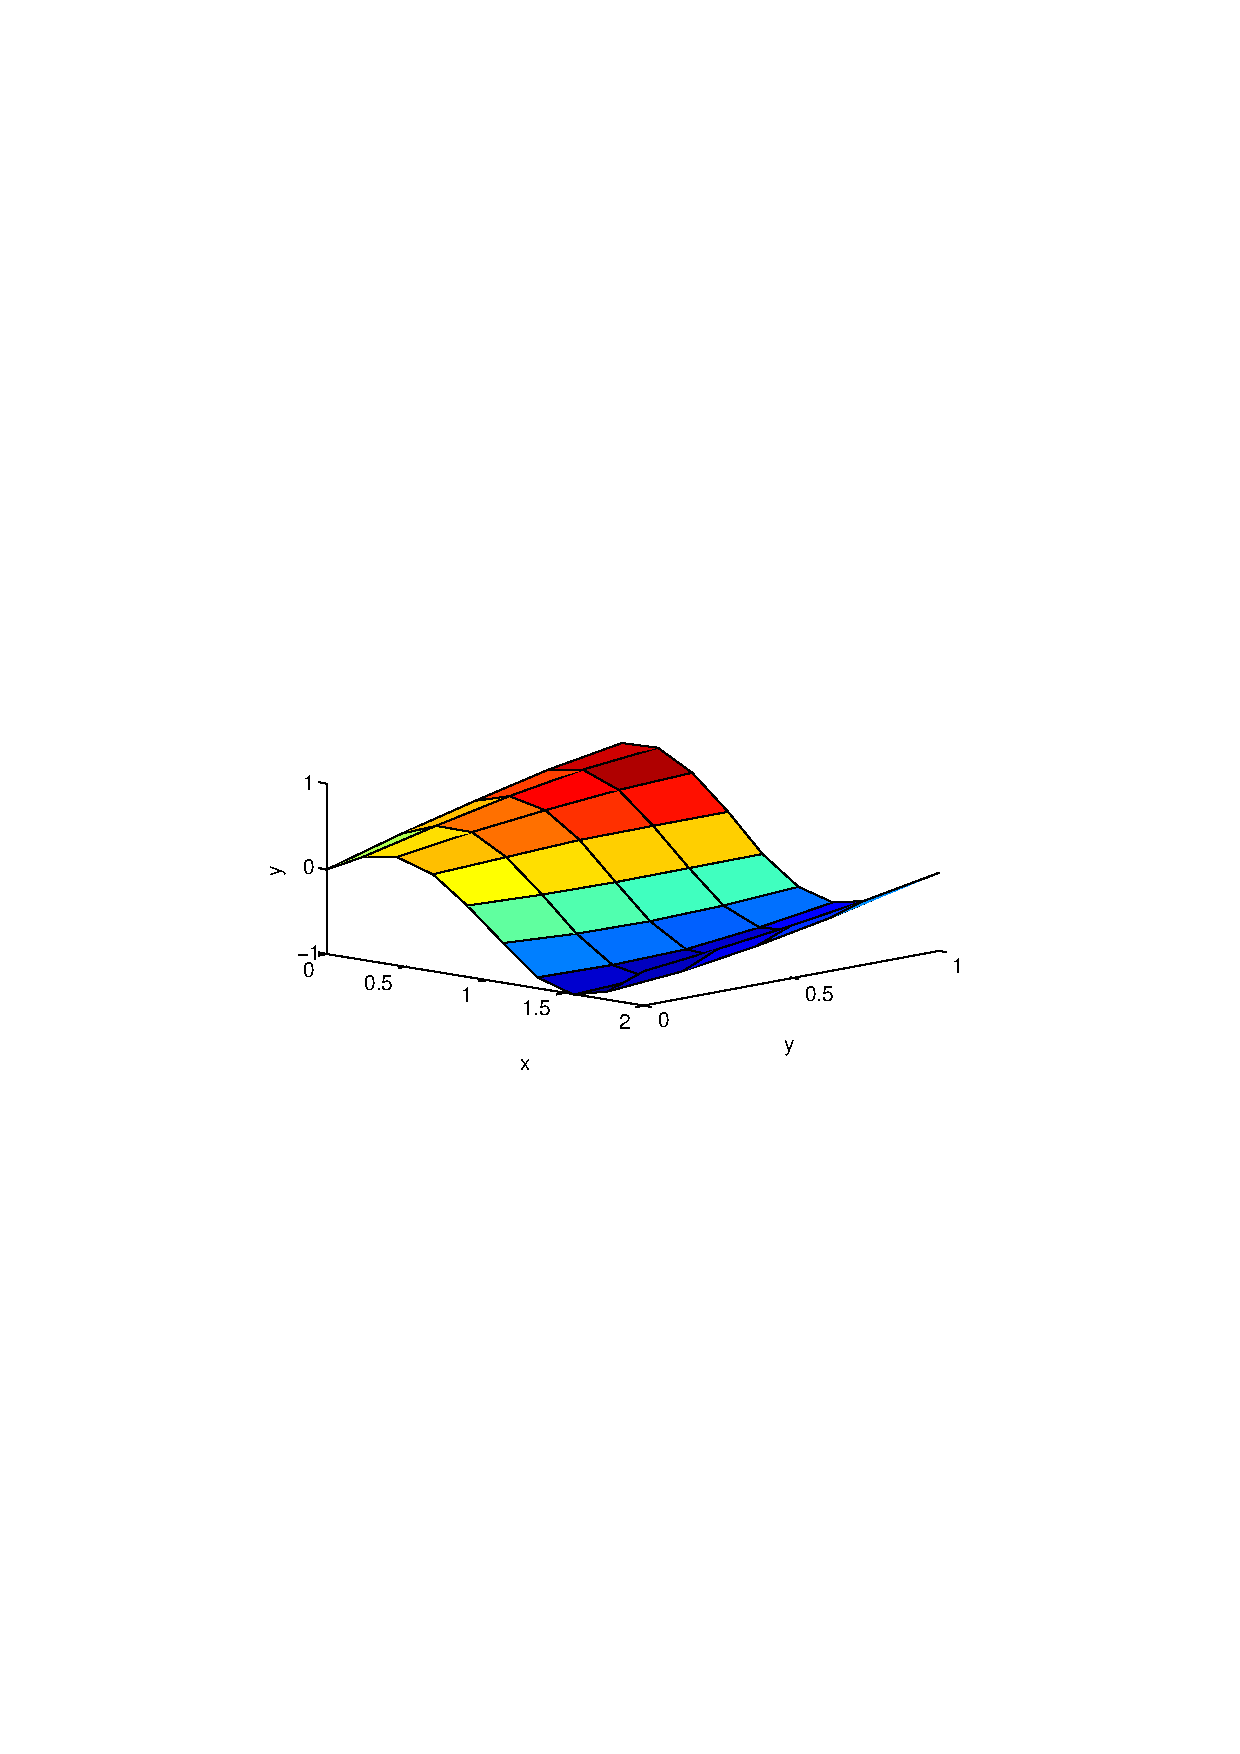
\includegraphics[width=0.45\linewidth, trim=3cm 11cm 3cm 11cm]{chapters/theory/X.pdf}
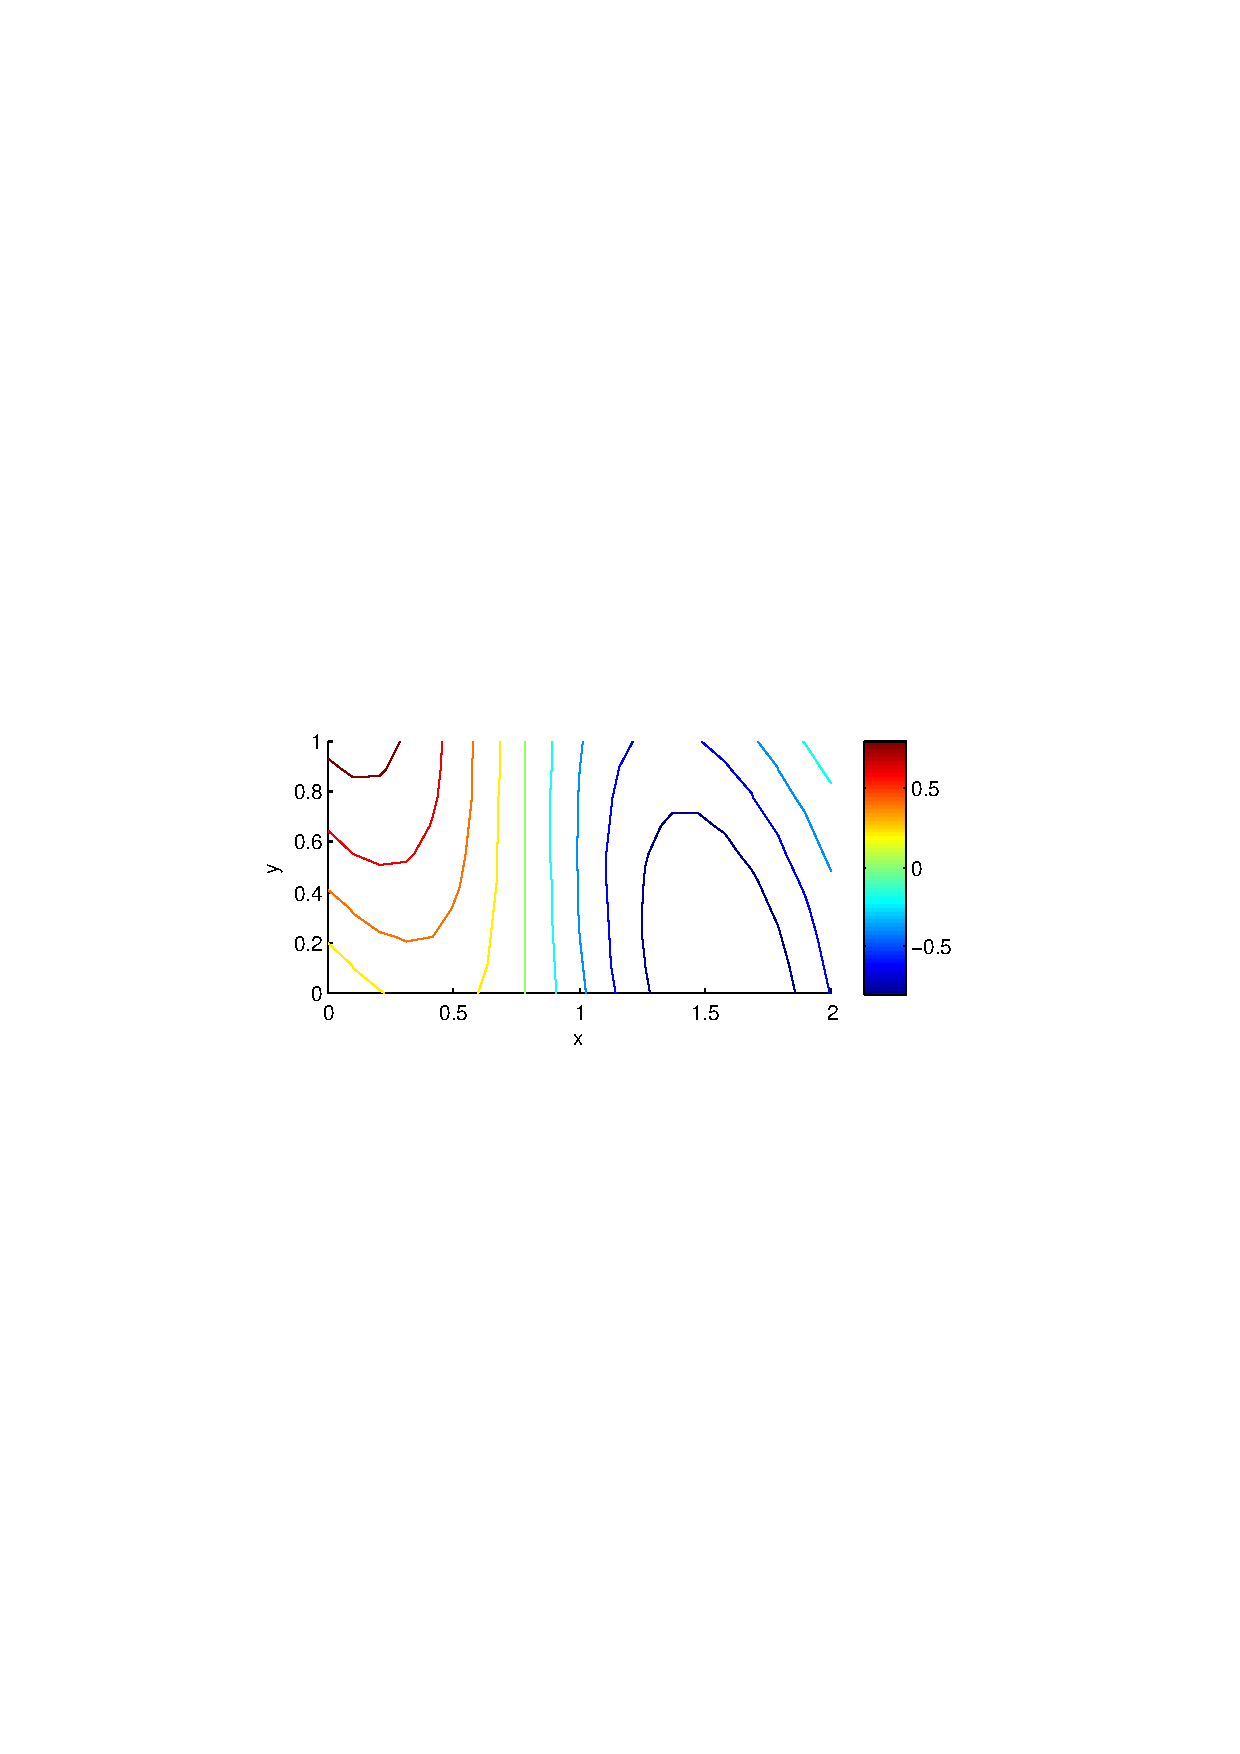
\includegraphics[width=0.45\linewidth, trim=3cm 11cm 3cm 11cm]{chapters/theory/Y.pdf}
\caption{Surface and contour plots showing the two dimensional function $z(x,y)=\sin(x+y)\cos(2x)$.}
\end{figure}

\section{Equation}
\begin{equation}
f(t)=\left\{ \begin{array}{ll}
1,~~~~ & t< 1 \\
t^2 & t\geq 1
\end{array}\right.
\end{equation}

\section{Table}
\begin{table}[H]
\centering
\caption{Values of $f(t)$ for $t=0,1,\dots 5$.}
\begin{tabular}{l|llllll} \hline\hline
$t$ & 0 & 1 & 2 & 3 & 4 & 5 \\ \hline
$f(t)$ & 1 & 1 & 4 & 9 & 16 & 25 \\ \hline\hline
\end{tabular}
\end{table}

\section{Chemical structure}
\begin{center}
\chemfig{X*5(-E-T-A-L-)}
\end{center}

\section{List}
\begin{enumerate}
  \item The first item
  \begin{enumerate}
    \item Nested item 1
    \item Nested item 2
  \end{enumerate}
  \item The second item
  \item The third item
  \item \dots
\end{enumerate}

\section{Source code listing}
%\lstset{language=Matlab}
\begin{lstlisting}[frame=single]
% Generate x- and y-nodes
x=linspace(0,1); y=linspace(0,1);

% Calculate z=f(x,y)
for i=1:length(x)
 for j=1:length(y)
  z(i,j)=x(i)+2*y(j);
 end
end
\end{lstlisting}

\section{To-do note}
The \texttt{todo} package enables to-do notes to be added in the page margin. This can be a very convenient way of making notes in the document during the process of writing. All notes can be hidden by using the option \emph{disable} when loading the package in the settings. \todo{Example of a to-do note.}


\chapter{Methods}
\lipsum[1-10]

\chapter{Results}
\lipsum[1-3]
\cite{Einstein:1905} % to get bib entry

\chapter{Conclusion}
\lipsum[1]


% REFERENCES / BIBLIOGRAPHY
% Use a separate file to be able to exclude with \includeonly
% \nocite{*}
\printbibliography[title={\thesisBibName}, heading=bibintoc]


% APPENDICES
\appendix
% CREATED BY MAGNUS GUSTAVER, 2020
\chapter{First Appendix}
\lipsum[1]

\chapter{Second Appendix}
\lipsum[1]


% LAST PAGE
\if\thesisStatus f
    % LAST PAGE
{ % make parskip changes local
\if\thesisLayout 2 % place lastpage correctly
    \cleardoublepage
    \pagenumbering{gobble}
    \newpage
    \thispagestyle{empty}
    \mbox{}
\else
    \pagenumbering{gobble}
\fi

\newpage
\thispagestyle{empty}

%Header Last Page
\vtop{
    \null\vspace{-27.5mm}
    \centerline{\textcolor{thesisHeaderColor}{\rule{1.28\textwidth}{28mm}}}
    \null\vspace{-9mm}
    \centerline{\textcolor{headerBrown}{\rule{1.28\textwidth}{4pt}}}
    \vspace{187mm}
    \if\thesisType M
    \centerline{
\includegraphics[width=0.2\pdfpagewidth]{template/figures/AvancezChalmersU_black_centered.eps}}
    \fi
    \if\thesisType B
    \centerline{
\includegraphics[width=0.2\pdfpagewidth]{template/figures/AvancezChalmers_black_centered.eps}}
    \fi
    \vspace{-220mm}
}

%\addtolength{\voffset}{2cm}
\renewcommand{\familydefault}{\sfdefault} \normalfont % Set cover page font
\pagestyle{empty}
\vspace*{-4.5cm}
\noindent
\textcolor{white}{\footnotesize \textbf{\MakeUppercase{\thesisDepartment}}\\
\textbf{\MakeUppercase{\thesisUniversity}} \\
\thesisLocation \\
\href{\thesisUniversityURL}{\textcolor{white}{\thesisUniversityURL}}}
}

\fi

\end{document}
